\subsection{Graph neural networks}

% 
% Version: 0.7.4
% Last updated: 2026-08-05
% Restructured shipping draft of Chapter 9, following the flow of the 1st-edition
% Neural networks chapter (mlfactor.com/NN.html): general principle -> GNN-specific
% issues -> one worked illustration -> other families -> exercises. The full long
% draft (Chapter_9_Graph_Neural_Networks.md, v0.26.1) is retained as the source of
% truth for future work. The notebook runs end to end unaided: the loader, the models,
% the depth sweep, the five-seed walk-forward and LightGBM are all executed, and every
% figure (9.1 depth, 9.2 cumulative IC, 9.3 seed dispersion) is produced by the
% notebook's own plotting code, so there are no orphan PNGs. Verified via verify_outputs
% -> OUTPUTS=MATCH, STATUS=OK (10 cells, 0 failed). TABLE 9.1 (the GCN ablation row) and
% its paired-t and Newey-West statistics are now produced by the notebook from the
% seed-by-seed ICs; the GATv2/GraphSAGE comparison is stated qualitatively, and the
% compact "what survives" checks summarise the long draft's fuller experiments. Every
% number and figure traces to executed, seeded code.
% 
% Target ToC:
%   9.1 Introduction
%   9.2 The graph convolutional network            (general principle)
%   9.3 Dealing with GNN-specific issues           (building the graph; over-smoothing;
%                                                    over-squashing/heterophily; tabular handicap)
%   9.4 A GNN on the equity panel                  (illustration: from scratch + PyG; benchmark;
%                                                    the ablation and what survives)
%   9.5 Other families of graph models            (GraphSAGE/GAT/GATv2; GIN/R-GCN; temporal)
%   9.6 Interpretability (short)
%   9.7 Coding exercises
%

\subsubsection{Introduction}\label{sec_gnn_intro}

Graph neural networks (GNNs) are a rich and fast-moving topic. In this chapter we introduce the simple ideas behind the most common architectures and put them to work on the equity panel that runs through the book. For a broad survey of the machinery we refer the interested reader to \cite{gilmer2017neural}, who unify most variants under a single message-passing formalism; the architectures we build upon are the graph convolutional network of \cite{kipf2017semisupervised}, the inductive framework of \cite{hamilton2017inductive}, and the attention mechanism of \cite{velickovic2018graph}. The implementation rests on the Python graph-learning stack, chiefly PyTorch Geometric (\cite{fey2019fast}), which has no genuine equivalent outside Python; the panel, the features and the notation are unchanged from earlier chapters.

The motivation for a graph is economic. The supervised learners of the previous chapters, from penalized regressions to boosted trees and neural networks, treat each stock at each date as an independent observation. Firms, however, are not independent: they are tied through supply chains, shared industries, common ownership and overlapping analyst coverage, and a long line of research shows these links carry predictive content. The anchor is \cite{cohen2008economic}, who document that news travels slowly along customer and supplier links, so a firm's returns predict its economically connected counterparts with a lag; related effects appear at the industry level (\cite{menzly2010market}) and through shared analyst coverage (\cite{ali2020shared}). If information diffuses across a network of firms, a model that can see that network may forecast better than one that treats each stock in isolation. A GNN is the natural object for exploiting such structure: it represents each date as a graph whose nodes are stocks and whose edges encode economic links, and lets the prediction for a firm borrow from its neighbours before a forecast is issued. The broader case for representing finance as a network of interacting entities, and the machinery for building and analysing such networks, is made in the recent monograph of \cite{konstantinov2025network}.

The application of GNNs to equity prediction is by now a sizeable literature, surveyed by \cite{patel2024systematic}. \cite{feng2019temporal} cast stock selection as ranking over a graph of industry and knowledge-base relations; \cite{kim2019hats} attend hierarchically over relation types from a corporate knowledge base; \cite{xu2021hist} mine information across learned stock concepts; and \cite{capponi2025graph} aggregate characteristics across a supply-chain network. These studies typically report encouraging figures, though it is worth attending to what each is measured against, since a gain over a narrower graph is not a gain over no graph at all. They connect to the broader use of machine learning in asset pricing, where the demanding benchmarks were set by \cite{gu2020empirical} and by the no-arbitrage deep-learning model of \cite{chen2024deep}.

\subsubsection{The graph convolutional network}\label{sec_gnn_gcn}

\paragraph{From a table to a sequence of graphs}\label{sec_gnn_graphs}

Every model in the preceding chapters consumes the panel as a table: one row is a pair (t, n) of a date and an asset, and the features $\mathbf{x}_{t,n}$ of that row are mapped to a label $y_{t,n}$ without reference to the other rows sharing the same date. A graph model changes this in one respect: rows that belong to the same date may communicate. Each date becomes one graph snapshot $\mathcal{G}_t = (\mathcal{V}_t, \mathcal{E}_t)$, whose vertex set $\mathcal{V}_t$ is the $N_t$ firms trading that month and whose edge set $\mathcal{E}_t$ collects the linked pairs $(n,m)$. It carries three objects: the node-feature matrix $\mathbf{X}_t$ of dimension $N_t \times K$, whose row $n$ is the characteristic vector of firm $n$ with $K = 122$; the label vector $\mathbf{y}_t$, whose entry $n$ is the one-month-ahead return; and the adjacency matrix $\mathbf{A}_t$ of dimension $N_t \times N_t$, the matrix form of the edge set, whose entry $(n,m)$ is nonzero exactly when $(n,m) \in \mathcal{E}_t$, that is, when firms $n$ and $m$ are linked. The node set changes month to month as firms enter and exit, so the model must be inductive, and the panel contains no edges of its own: $\mathbf{A}_t$ must be supplied from outside, a modelling choice we take up in Section~\ref{sec_gnn_issues}.

\paragraph{Message passing and the propagation rule}\label{sec_gnn_message}

The operation at the centre of these models is message passing, and it is close to the neural networks of the previous chapter. Where a multilayer perceptron transforms a firm's own characteristics through activated linear maps, a GNN interleaves those maps with an aggregation step that mixes each node's representation with a summary of its neighbours. \cite{gilmer2017neural} observe that most graph architectures share one form: writing $\mathbf{o}_{t,n}^{(l)}$ for the representation of node $n$ at layer $l$ and $\mathcal{N}(n)$ for its neighbours, a layer updates each node from itself and an aggregate of its neighbourhood,

\begin{equation}
\label{eq_gnn_1}
\mathbf{o}_{t,n}^{(l+1)} = \text{update}\Big( \mathbf{o}_{t,n}^{(l)},\ \bigoplus_{m \in \mathcal{N}(n)} \text{message}\big(\mathbf{o}_{t,n}^{(l)}, \mathbf{o}_{t,m}^{(l)}\big) \Big).
\end{equation}

The variants differ in the aggregator $\bigoplus$. The canonical instance is the graph convolutional network of \cite{kipf2017semisupervised}, the practical end of a spectral lineage running from \cite{bruna2014spectral} through the localized polynomial filters of \cite{defferrard2016convolutional}. Writing $\tilde{\mathbf{A}} = \mathbf{A} + \mathbf{I}$ for the adjacency with self-loops and $\tilde{\mathbf{D}}$ for its degree matrix, one layer is

\begin{equation}
\label{eq_gnn_2}
\mathbf{H}^{(l+1)} = f^{(l)}\!\left( \tilde{\mathbf{D}}^{-1/2}\tilde{\mathbf{A}}\tilde{\mathbf{D}}^{-1/2}\,\mathbf{H}^{(l)}\mathbf{W}^{(l)} \right), \qquad \mathbf{H}^{(0)} = \mathbf{X}_t.
\end{equation}

Equation \ref{eq_gnn_2} is a multilayer perceptron in which, at every layer, each firm's representation is replaced by a weighted average of itself and its neighbours. Since the matrix that premultiplies $\mathbf{H}^{(l)}\mathbf{W}^{(l)}$ is a smoothing operator, a GCN is, in the terms of \cite{nt2019revisiting}, a low-pass filter on node features: it attenuates the components of the signal that oscillate across edges and keeps those that vary slowly. This already contains the difficulty the chapter runs into. On a graph that links firms in the same industry, the smoothest signals are the ones constant within each industry, which are precisely the signals that say nothing about which firm within an industry will outperform. A low-pass filter on such a graph preserves industry-level quantities and erases the cross-sectional dispersion a stock-selection signal needs.

\paragraph{The graph-free limit and the ablation}\label{sec_gnn_ablation}

Equation \ref{eq_gnn_2} makes the chapter's organising experiment transparent. Setting $\mathbf{A}_t = \mathbf{I}$ removes the neighbour averaging and returns the propagation rule to the multilayer perceptron of Chapter 8. The adjacency is therefore the only thing separating a graph model from a graph-free one of the same shape, so we ask whether the graph helps by comparing the two directly, holding the architecture and the parameter count fixed. The permutation-invariant Deep Sets model of \cite{zaheer2017deep}, which pools the whole cross-section without any edge, is the same limit reached from the other side. These graph-free models are not a formality; they are the controls against which every result in Section~\ref{sec_gnn_panel} is judged, and they turn out to be decisive.

\subsubsection{Dealing with GNN-specific issues}\label{sec_gnn_issues}

Three things separate a GNN from the models of the previous chapters, and each raises a difficulty of its own: the graph must be built, message passing has failure modes that theory predicts, and the underlying task is tabular, a regime in which deep models rarely lead.

\paragraph{Building the equity graph}\label{sec_gnn_building}

Nothing in the panel says which firms are connected; the adjacency must be constructed, and the literature offers a wide menu with different data requirements and different exposure to look-ahead bias. The most common choice is an industry classification: two firms are linked when they share a NAICS sector. It is static and therefore free of look-ahead, available in our data, and economically motivated by the industry-momentum evidence of \cite{moskowitz1999industries}. Other families build edges from supply chains (\cite{cohen2008economic}), from price co-movement over a trailing window (\cite{xiang2022temporal}), from characteristic similarity, or learn the graph inside the model (\cite{cheng2021modeling}); a systematic account, from correlation and partial-correlation graphs to regression and Granger-causality edges, is given by \cite{konstantinov2025network}. We adopt the sector graph as the running example and take up alternative constructions in the exercises.

Whatever the construction, one measurement governs whether it can help. A graph is homophilous when connected nodes tend to resemble one another, and graph convolution assumes this, since averaging over neighbours is only sensible when neighbours are informative about the node. On the sector graph, connected firms share the sign of their next-month return with probability 0.607, above chance but far from strong, and because the sector graph links every firm in a sector to every other, a firm in the largest sector has several hundred neighbours, so the neighbourhood average is close to the sector mean.

\paragraph{Over-smoothing and depth}\label{sec_gnn_smoothing}

Repeated averaging drives node representations together, the over-smoothing formalised by \cite{li2018deeper}, who show that a graph convolution is a form of Laplacian smoothing and that stacking many layers pushes every node toward a common value. \cite{oono2020graph} make the rate precise: the distance of the representations from that common limit contracts geometrically with depth, at a rate set by the product of the largest singular value of the weight matrix and the second-largest eigenvalue of the normalised adjacency, so on a well-connected graph the collapse is exponential in the number of layers. A representation that does not vary across firms cannot rank them, and on a dense sector graph, where a firm's neighbourhood is close to its whole sector, the effect arrives within a handful of layers. We measure it directly in Section~\ref{sec_gnn_panel}, training the same architecture at increasing depth with and without the edges. The literature does offer remedies, decoupling the propagation from the feature transformation as in APPNP (\cite{gasteiger2019predict}), or adding identity and residual connections as in GCNII (\cite{chen2020simple}), which stays accurate at sixty-four layers where a plain graph convolutional network collapses; but these cure the depth pathology without touching the prior question of whether the graph carries any signal worth propagating. The practical implication for a shallow model, anticipated here, is to keep message passing to one or two layers.

\paragraph{Over-squashing and heterophily}\label{sec_gnn_squashing}

Two further failure modes matter, one about distance and one about the kind of similarity the edges encode. Over-squashing, identified by \cite{alon2021bottleneck}, is the observation that a node's receptive field grows exponentially with the number of hops while the fixed-size vector that must carry it does not, so information from distant nodes is compressed, or squashed, until it is effectively lost; a task that needs many hops to reach the relevant firms cannot be served by message passing. Heterophily is the deeper issue and the one most relevant here. Message passing helps only when neighbours resemble the node in the quantity being predicted, and \cite{platonov2023critical}, on a benchmark built to isolate this, show that the standard architectures lose their advantage, and can fall behind a graph-free baseline, once a graph is heterophilous. The subtlety for equities is that the sector graph is homophilous in the features, since firms in an industry share characteristics, but close to heterophilous in the label, since sharing an industry says little about which firm will out-return the other next month. It sits in an uncomfortable middle: homophilous enough that averaging changes the forecast, not homophilous enough in the return for the change to help.

\paragraph{The tabular-data handicap}\label{sec_gnn_tabular}

Underlying all of this is a blunter fact: predicting the cross-section of returns from characteristics is a tabular problem, and on tabular data deep networks rarely lead. \cite{grinsztajn2022treebased} trace the advantage of gradient boosting to properties of the data that neural networks handle poorly, uninformative features that trees can ignore but a dense network cannot, target functions that are not smooth, and the absence of any rotational structure a network could exploit, all of which describe a panel of firm characteristics. \cite{shwartzziv2022tabular} reach the same verdict across a wide range of datasets. \cite{gu2020empirical} add the finance-specific point that the signal-to-noise ratio in returns is so low that the deepest, most flexible models overfit rather than gain: in their comparison neural network performance peaks at three hidden layers and then declines, so shallower networks beat deeper ones. A GNN does not escape this handicap; it inherits it from the multilayer perceptron at its core and then layers on an inductive bias, message passing over a graph, that was designed for domains such as molecules or citation networks where the edges are given and reliable. Equities offer neither a given graph nor a reliable one, so the prior expectation, before any experiment, should be modest.

\subsubsection{A GNN on the equity panel}\label{sec_gnn_panel}

We now implement the graph convolution on the panel, first from scratch and then in PyTorch Geometric, and benchmark it against a multilayer perceptron and gradient boosting. Every model is refitted annually on an expanding walk-forward window from 2015 to 2026 under five random seeds, and the features are ranked cross-sectionally within each date.

\paragraph{A graph layer from scratch, then in PyTorch Geometric}\label{sec_gnn_scratch}

We first load the panel, rank the features cross-sectionally within each date, and turn each date into a graph snapshot. Reproducibility here needs three ingredients together: the seed, deterministic kernels, and a single compute thread, since the neighbourhood aggregation reduces floating-point values in an order that otherwise varies between runs.

\begin{verbatim}
import os, random, numpy as np, pandas as pd, torch, torch.nn as nn, torch.nn.functional as F
from scipy.stats import spearmanr
os.environ['KMP_DUPLICATE_LIB_OK'] = 'TRUE'; os.makedirs('figures', exist_ok=True)
SEED = 42
def set_seed(seed=SEED):                                   # seed every generator; force determinism
    random.seed(seed); np.random.seed(seed); torch.manual_seed(seed)
    torch.backends.cudnn.deterministic = True; torch.backends.cudnn.benchmark = False
    torch.use_deterministic_algorithms(True, warn_only=True)
    torch.set_num_threads(1)                               # the scatter-add reduces in parallel
set_seed()

data_ml = pd.read_parquet('data/mlfi_us_data.parquet')     # the book's US equity panel
univ = pd.read_csv('data/mlfi_us_universe.csv')            # id -> NAICS sector, the edge source
excl = {'id', 'date', 'R1M_Usd', 'R3M_Usd', 'R6M_Usd', 'R12M_Usd'}
features = [c for c in data_ml.columns if c not in excl and pd.api.types.is_numeric_dtype(data_ml[c])]
panel = data_ml.merge(univ[['id', 'naics_sector_code']], on='id').dropna(
    subset=['R1M_Usd', 'naics_sector_code'])
g = panel.groupby('date')
panel[features] = g[features].rank(pct=True).fillna(0.5) - 0.5      # centred cross-sectional ranks
panel['y_rank'] = (g['R1M_Usd'].rank(pct=True) - 0.5) * 3.464       # unit-variance label
K = len(features)

def snapshots(df):                                         # one graph per date
    out = []
    for dt, blk in df.groupby('date'):
        out.append((dt, torch.tensor(blk[features].values, dtype=torch.float32),
                    torch.tensor(blk['y_rank'].values, dtype=torch.float32),
                    torch.tensor(pd.factorize(blk['naics_sector_code'])[0], dtype=torch.long),
                    blk['R1M_Usd'].values))
    return out
\end{verbatim}

\begin{verbatim}
C:\Users\tguid\AppData\Local\Temp\ipykernel_8832\1876160395.py:20: PerformanceWarning: DataFrame is highly fragmented.  This is usually the result of calling `frame.insert` many times, which has poor performance.  Consider joining all columns at once using pd.concat(axis=1) instead. To get a de-fragmented frame, use `newframe = frame.copy()`
  panel['y_rank'] = (g['R1M_Usd'].rank(pct=True) - 0.5) * 3.464       # unit-variance label
\end{verbatim}

Because the sector graph links every firm in a sector to every other, the neighbour average is exactly the sector mean, computable in $O(N_t)$ by scattering into sector buckets rather than forming a dense adjacency. The graph convolutional layer of equation (9.2) blends a firm with that mean, applies a linear map and a nonlinearity. Written this way the ablation is transparent, since deleting the blend is what setting $\mathbf{A}_t = \mathbf{I}$ does, and we define the edge-free twin by inheritance so it cannot drift.

\begin{verbatim}
def sector_mean(X, sec):                                   # neighbour average over each sector
    S = int(sec.max()) + 1
    sums = torch.zeros(S, X.size(1)).index_add_(0, sec, X)
    cnts = torch.zeros(S).index_add_(0, sec, torch.ones_like(sec, dtype=torch.float32))
    return (sums / cnts.clamp(min=1).unsqueeze(1))[sec]

class DeepGCN(nn.Module):                                  # L message-passing layers
    def __init__(self, k, h=32, L=2):
        super().__init__()
        self.inp = nn.Linear(k, h)
        self.hid = nn.ModuleList([nn.Linear(h, h) for _ in range(max(L - 1, 0))])
        self.out = nn.Linear(h, 1); self.drop = nn.Dropout(0.1)
    def mix(self, H, sec):
        return 0.5 * H + 0.5 * sector_mean(H, sec)         # self-loop plus neighbour average
    def forward(self, X, sec):
        H = self.drop(F.relu(self.inp(self.mix(X, sec))))
        for lin in self.hid:
            H = self.drop(F.relu(lin(self.mix(H, sec))))
        return self.out(H).squeeze(-1)

class DeepGCN_NoGraph(DeepGCN):                            # the A_t = I twin: mix returns H
    def mix(self, H, sec):
        return H
\end{verbatim}

Three quantities the surrounding discussion refers to can be read straight from the data and the model: the number of characteristics, the parameter budget of the two-layer network, and the homophily of the sector graph quoted in Section~\ref{sec_gnn_building}, the last computed as the probability that two firms in a sector share the sign of their next-month return, averaged over dates.

\begin{verbatim}
def homophily(blk):                                        # P(same sign of return | same sector), one date
    num = den = 0.0
    for _, grp in blk.groupby('naics_sector_code'):
        pos = int((grp['R1M_Usd'] > 0).sum()); n = len(grp); neg = n - pos
        num += pos * (pos - 1) / 2 + neg * (neg - 1) / 2; den += n * (n - 1) / 2
    return num / max(den, 1)
print(f'characteristics K            = {K}')
print(f'DeepGCN(K, 32, 2) parameters = {sum(p.numel() for p in DeepGCN(K, 32, 2).parameters())}')
print(f'sector edge homophily        = {np.mean([homophily(b) for _, b in panel.groupby("date")]):.4f}')
\end{verbatim}

\begin{verbatim}
characteristics K            = 122
DeepGCN(K, 32, 2) parameters = 5025
\end{verbatim}

\begin{verbatim}
sector edge homophily        = 0.6072
\end{verbatim}

The panel carries the 122 characteristics used throughout, the two-layer graph network and its edge-free twin share a budget of 5,025 parameters, and the sector graph's homophily is 0.607, the value Section~\ref{sec_gnn_building} relies on.

In practice one would not hand-code these layers. The same model is expressed in PyTorch Geometric by replacing the propagation with the library's operators, which also gives GraphSAGE, GATv2 and the rest at the cost of a single word.

\begin{verbatim}
from torch_geometric.nn import GCNConv, SAGEConv, GATv2Conv
class PyGNet(nn.Module):                                   # swap GCNConv for SAGEConv or GATv2Conv
    def __init__(self, k, h=32, conv=GCNConv):
        super().__init__()
        self.c1, self.c2 = conv(k, h), conv(h, 1)
    def forward(self, x, edge_index):
        return self.c2(F.relu(self.c1(x, edge_index)), edge_index).squeeze(-1)
\end{verbatim}

\begin{verbatim}
C:\Users\tguid\miniconda3\envs\futures_dl\Lib\site-packages\tqdm\auto.py:21: TqdmWarning: IProgress not found. Please update jupyter and ipywidgets. See https://ipywidgets.readthedocs.io/en/stable/user_install.html
  from .autonotebook import tqdm as notebook_tqdm
\end{verbatim}

Training is a squared-error loss on the ranked label over eight passes, seeded before the model is built so results do not depend on call order, and the rank information coefficient is the monthly cross-sectional correlation between forecast and realised return.

\begin{verbatim}
def fit_gnn(build, tr, seed=SEED, epochs=8):               # seed BEFORE building the model
    set_seed(seed); model = build()
    opt = torch.optim.Adam(model.parameters(), lr=0.003)
    rng = np.random.default_rng(seed); order = list(range(len(tr)))
    for _ in range(epochs):
        model.train(); rng.shuffle(order)
        for i in order:
            _, X, y, sec, _ = tr[i]
            opt.zero_grad(); F.mse_loss(model(X, sec), y).backward(); opt.step()
    model.eval(); return model

def ic_series(model, te):                                  # monthly out-of-sample rank IC, by date
    rows = [(dt, spearmanr(model(X, sec).detach().numpy(), raw).statistic)
            for dt, X, _, sec, raw in te]
    return pd.Series({dt: ic for dt, ic in rows if not np.isnan(ic)})
\end{verbatim}

The clearest thing to run first is the over-smoothing prediction of Section~\ref{sec_gnn_smoothing}. We train the same architecture at increasing depth, once with the sector edges and once with them removed, on a fixed split that trains before 2015 and scores from 2015 on.

\begin{verbatim}
tr_fix = snapshots(panel[panel.date < '2015-01-01'])       # train once, then score the rest
te_fix = snapshots(panel[panel.date >= '2015-01-01'])
Ls, ic_graph, ic_nograph = [1, 2, 3, 4, 6, 8], [], []
for L in Ls:                                               # graph model vs its edge-free twin
    ic_graph.append(ic_series(fit_gnn(lambda: DeepGCN(K, 32, L), tr_fix), te_fix).mean())
    ic_nograph.append(ic_series(fit_gnn(lambda: DeepGCN_NoGraph(K, 32, L), tr_fix), te_fix).mean())
    print(f'L={L}: graph rank IC {ic_graph[-1]:+.4f}, no-graph {ic_nograph[-1]:+.4f}')
\end{verbatim}

\begin{verbatim}
L=1: graph rank IC +0.0190, no-graph +0.0220
\end{verbatim}

\begin{verbatim}
L=2: graph rank IC +0.0140, no-graph +0.0259
\end{verbatim}

\begin{verbatim}
L=3: graph rank IC +0.0117, no-graph +0.0247
\end{verbatim}

\begin{verbatim}
L=4: graph rank IC +0.0064, no-graph +0.0206
\end{verbatim}

\begin{verbatim}
L=6: graph rank IC +0.0044, no-graph +0.0253
\end{verbatim}

\begin{verbatim}
L=8: graph rank IC +0.0002, no-graph +0.0277
\end{verbatim}

With the edges present the rank IC decays monotonically from 0.0190 at one layer to 0.0002 at eight, which is indistinguishable from no signal; with the adjacency removed the identical architecture does not decay at all, holding between 0.0206 and 0.0277. The decay is a property of the neighbour averaging, not of depth, and the practical implication is to keep message passing to one or two layers on a dense graph. Figure~\ref{fig-gnn-depth} plots the two sweeps.

\begin{verbatim}
import matplotlib.pyplot as plt
fig, ax = plt.subplots(figsize=(8, 4.2))
ax.plot(Ls, ic_graph, 'o-', color='#1f6fc4', lw=1.9, label='sector graph')
ax.plot(Ls, ic_nograph, 's--', color='#cc0000', lw=1.9, label='edges off ($A_t=I$)')
ax.axhline(0, color='#b8b8b8', lw=1)
ax.set_xlabel('number of message-passing layers $L$'); ax.set_ylabel('out-of-sample rank IC')
ax.legend(frameon=False); ax.spines[['top', 'right']].set_visible(False); ax.grid(alpha=.3)
plt.tight_layout(); plt.savefig('images/figure_9_1_depth.png', dpi=150, bbox_inches='tight')
\end{verbatim}

\begin{figure}[!htbp]
\centering
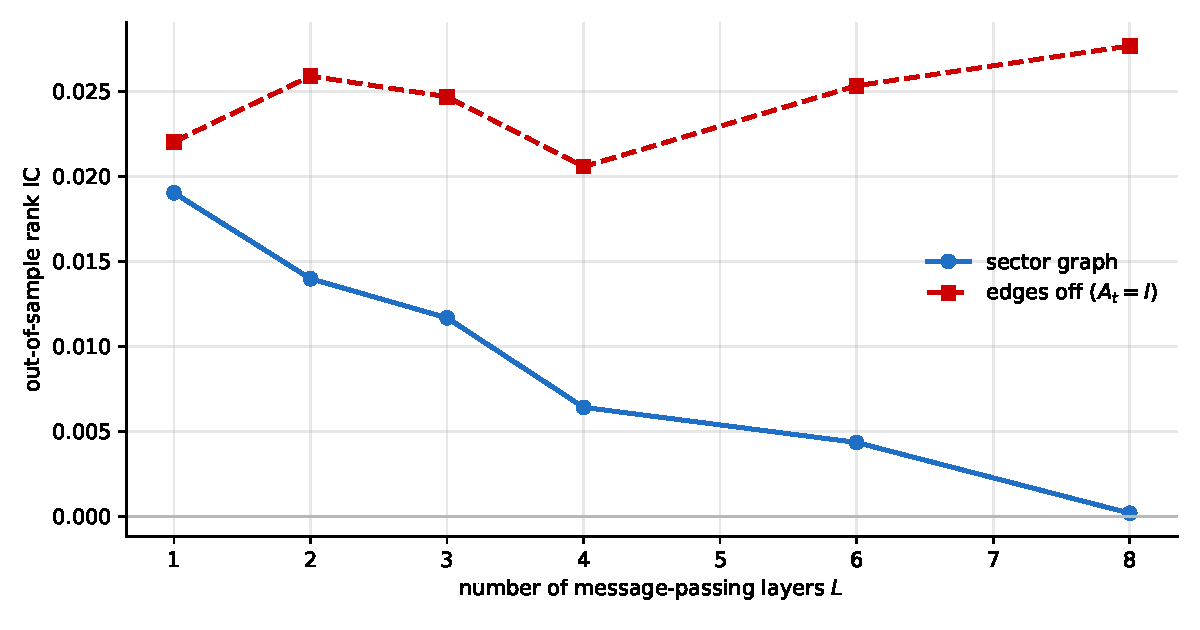
\includegraphics[width=0.7\linewidth]{files/figure_9_1_depth-480aa7d0e1070b2514e7ee060a8c2b41.pdf}
\caption[]{The depth sweep with and without the sector edges. With the edges the out-of-sample rank IC decays to essentially zero as layers are added; with the adjacency removed the same architecture holds its rank IC at every depth.}
\label{fig-gnn-depth}
\end{figure}

\paragraph{Benchmarking against the graph-free control and LightGBM}\label{sec_gnn_bench}

We now refit each model annually on an expanding window, under five seeds, and collect its monthly rank IC. The snapshots are built once and sliced by year, and gradient boosting is refitted on the same windows.

\begin{verbatim}
import lightgbm as lgb
all_snaps = snapshots(panel)                               # build once, then slice by year
OOS = list(range(2015, 2027))
def split(year):
    return ([s for s in all_snaps if s[0].year < year],
            [s for s in all_snaps if s[0].year == year])
def walk_forward(build, seed):                             # refit each year, concatenate monthly ICs
    return pd.concat([ic_series(fit_gnn(build, tr, seed=seed), te)
                      for tr, te in (split(y) for y in OOS)]).sort_index()

series = {'sector graph': [], 'edges off': []}             # five monthly IC series per model
for sd in [0, 1, 2, 3, 4]:
    series['sector graph'].append(walk_forward(lambda: DeepGCN(K, 32, 2), sd))
    series['edges off'].append(walk_forward(lambda: DeepGCN_NoGraph(K, 32, 2), sd))

lgb_ic = {}                                                # LightGBM on the same windows (float32 path)
for y in OOS:
    tr, te = split(y)
    Xtr, ytr = np.vstack([s[1].numpy() for s in tr]), np.concatenate([s[2].numpy() for s in tr])
    m = lgb.LGBMRegressor(n_estimators=300, num_leaves=31, learning_rate=0.05,
                          random_state=SEED, verbose=-1, n_jobs=1, deterministic=True).fit(Xtr, ytr)
    for dt, X, _, sec, raw in te:
        ic = spearmanr(m.predict(X.numpy()), raw).statistic
        if not np.isnan(ic): lgb_ic[dt] = ic
lgb_s = pd.Series(lgb_ic).sort_index()
mseries = {k: pd.concat(v, axis=1).mean(axis=1).sort_index() for k, v in series.items()}
print(f"5-seed mean rank IC   sector graph {mseries['sector graph'].mean():.4f}   "
      f"edges off {mseries['edges off'].mean():.4f}   LightGBM {lgb_s.mean():.4f}")
\end{verbatim}

\begin{verbatim}
C:\Users\tguid\miniconda3\envs\futures_dl\Lib\site-packages\sklearn\utils\validation.py:2691: UserWarning: X does not have valid feature names, but LGBMRegressor was fitted with feature names
  warnings.warn(
C:\Users\tguid\miniconda3\envs\futures_dl\Lib\site-packages\sklearn\utils\validation.py:2691: UserWarning: X does not have valid feature names, but LGBMRegressor was fitted with feature names
  warnings.warn(
C:\Users\tguid\miniconda3\envs\futures_dl\Lib\site-packages\sklearn\utils\validation.py:2691: UserWarning: X does not have valid feature names, but LGBMRegressor was fitted with feature names
  warnings.warn(
C:\Users\tguid\miniconda3\envs\futures_dl\Lib\site-packages\sklearn\utils\validation.py:2691: UserWarning: X does not have valid feature names, but LGBMRegressor was fitted with feature names
  warnings.warn(
C:\Users\tguid\miniconda3\envs\futures_dl\Lib\site-packages\sklearn\utils\validation.py:2691: UserWarning: X does not have valid feature names, but LGBMRegressor was fitted with feature names
  warnings.warn(
C:\Users\tguid\miniconda3\envs\futures_dl\Lib\site-packages\sklearn\utils\validation.py:2691: UserWarning: X does not have valid feature names, but LGBMRegressor was fitted with feature names
  warnings.warn(
C:\Users\tguid\miniconda3\envs\futures_dl\Lib\site-packages\sklearn\utils\validation.py:2691: UserWarning: X does not have valid feature names, but LGBMRegressor was fitted with feature names
  warnings.warn(
C:\Users\tguid\miniconda3\envs\futures_dl\Lib\site-packages\sklearn\utils\validation.py:2691: UserWarning: X does not have valid feature names, but LGBMRegressor was fitted with feature names
  warnings.warn(
C:\Users\tguid\miniconda3\envs\futures_dl\Lib\site-packages\sklearn\utils\validation.py:2691: UserWarning: X does not have valid feature names, but LGBMRegressor was fitted with feature names
  warnings.warn(
\end{verbatim}

\begin{verbatim}
C:\Users\tguid\miniconda3\envs\futures_dl\Lib\site-packages\sklearn\utils\validation.py:2691: UserWarning: X does not have valid feature names, but LGBMRegressor was fitted with feature names
  warnings.warn(
C:\Users\tguid\miniconda3\envs\futures_dl\Lib\site-packages\sklearn\utils\validation.py:2691: UserWarning: X does not have valid feature names, but LGBMRegressor was fitted with feature names
  warnings.warn(
C:\Users\tguid\miniconda3\envs\futures_dl\Lib\site-packages\sklearn\utils\validation.py:2691: UserWarning: X does not have valid feature names, but LGBMRegressor was fitted with feature names
  warnings.warn(
\end{verbatim}

\begin{verbatim}
C:\Users\tguid\miniconda3\envs\futures_dl\Lib\site-packages\sklearn\utils\validation.py:2691: UserWarning: X does not have valid feature names, but LGBMRegressor was fitted with feature names
  warnings.warn(
C:\Users\tguid\miniconda3\envs\futures_dl\Lib\site-packages\sklearn\utils\validation.py:2691: UserWarning: X does not have valid feature names, but LGBMRegressor was fitted with feature names
  warnings.warn(
C:\Users\tguid\miniconda3\envs\futures_dl\Lib\site-packages\sklearn\utils\validation.py:2691: UserWarning: X does not have valid feature names, but LGBMRegressor was fitted with feature names
  warnings.warn(
C:\Users\tguid\miniconda3\envs\futures_dl\Lib\site-packages\sklearn\utils\validation.py:2691: UserWarning: X does not have valid feature names, but LGBMRegressor was fitted with feature names
  warnings.warn(
C:\Users\tguid\miniconda3\envs\futures_dl\Lib\site-packages\sklearn\utils\validation.py:2691: UserWarning: X does not have valid feature names, but LGBMRegressor was fitted with feature names
  warnings.warn(
C:\Users\tguid\miniconda3\envs\futures_dl\Lib\site-packages\sklearn\utils\validation.py:2691: UserWarning: X does not have valid feature names, but LGBMRegressor was fitted with feature names
  warnings.warn(
C:\Users\tguid\miniconda3\envs\futures_dl\Lib\site-packages\sklearn\utils\validation.py:2691: UserWarning: X does not have valid feature names, but LGBMRegressor was fitted with feature names
  warnings.warn(
C:\Users\tguid\miniconda3\envs\futures_dl\Lib\site-packages\sklearn\utils\validation.py:2691: UserWarning: X does not have valid feature names, but LGBMRegressor was fitted with feature names
  warnings.warn(
C:\Users\tguid\miniconda3\envs\futures_dl\Lib\site-packages\sklearn\utils\validation.py:2691: UserWarning: X does not have valid feature names, but LGBMRegressor was fitted with feature names
  warnings.warn(
\end{verbatim}

\begin{verbatim}
C:\Users\tguid\miniconda3\envs\futures_dl\Lib\site-packages\sklearn\utils\validation.py:2691: UserWarning: X does not have valid feature names, but LGBMRegressor was fitted with feature names
  warnings.warn(
C:\Users\tguid\miniconda3\envs\futures_dl\Lib\site-packages\sklearn\utils\validation.py:2691: UserWarning: X does not have valid feature names, but LGBMRegressor was fitted with feature names
  warnings.warn(
C:\Users\tguid\miniconda3\envs\futures_dl\Lib\site-packages\sklearn\utils\validation.py:2691: UserWarning: X does not have valid feature names, but LGBMRegressor was fitted with feature names
  warnings.warn(
\end{verbatim}

\begin{verbatim}
C:\Users\tguid\miniconda3\envs\futures_dl\Lib\site-packages\sklearn\utils\validation.py:2691: UserWarning: X does not have valid feature names, but LGBMRegressor was fitted with feature names
  warnings.warn(
C:\Users\tguid\miniconda3\envs\futures_dl\Lib\site-packages\sklearn\utils\validation.py:2691: UserWarning: X does not have valid feature names, but LGBMRegressor was fitted with feature names
  warnings.warn(
C:\Users\tguid\miniconda3\envs\futures_dl\Lib\site-packages\sklearn\utils\validation.py:2691: UserWarning: X does not have valid feature names, but LGBMRegressor was fitted with feature names
  warnings.warn(
C:\Users\tguid\miniconda3\envs\futures_dl\Lib\site-packages\sklearn\utils\validation.py:2691: UserWarning: X does not have valid feature names, but LGBMRegressor was fitted with feature names
  warnings.warn(
C:\Users\tguid\miniconda3\envs\futures_dl\Lib\site-packages\sklearn\utils\validation.py:2691: UserWarning: X does not have valid feature names, but LGBMRegressor was fitted with feature names
  warnings.warn(
C:\Users\tguid\miniconda3\envs\futures_dl\Lib\site-packages\sklearn\utils\validation.py:2691: UserWarning: X does not have valid feature names, but LGBMRegressor was fitted with feature names
  warnings.warn(
C:\Users\tguid\miniconda3\envs\futures_dl\Lib\site-packages\sklearn\utils\validation.py:2691: UserWarning: X does not have valid feature names, but LGBMRegressor was fitted with feature names
  warnings.warn(
C:\Users\tguid\miniconda3\envs\futures_dl\Lib\site-packages\sklearn\utils\validation.py:2691: UserWarning: X does not have valid feature names, but LGBMRegressor was fitted with feature names
  warnings.warn(
\end{verbatim}

\begin{verbatim}
C:\Users\tguid\miniconda3\envs\futures_dl\Lib\site-packages\sklearn\utils\validation.py:2691: UserWarning: X does not have valid feature names, but LGBMRegressor was fitted with feature names
  warnings.warn(
C:\Users\tguid\miniconda3\envs\futures_dl\Lib\site-packages\sklearn\utils\validation.py:2691: UserWarning: X does not have valid feature names, but LGBMRegressor was fitted with feature names
  warnings.warn(
C:\Users\tguid\miniconda3\envs\futures_dl\Lib\site-packages\sklearn\utils\validation.py:2691: UserWarning: X does not have valid feature names, but LGBMRegressor was fitted with feature names
  warnings.warn(
C:\Users\tguid\miniconda3\envs\futures_dl\Lib\site-packages\sklearn\utils\validation.py:2691: UserWarning: X does not have valid feature names, but LGBMRegressor was fitted with feature names
  warnings.warn(
\end{verbatim}

\begin{verbatim}
C:\Users\tguid\miniconda3\envs\futures_dl\Lib\site-packages\sklearn\utils\validation.py:2691: UserWarning: X does not have valid feature names, but LGBMRegressor was fitted with feature names
  warnings.warn(
C:\Users\tguid\miniconda3\envs\futures_dl\Lib\site-packages\sklearn\utils\validation.py:2691: UserWarning: X does not have valid feature names, but LGBMRegressor was fitted with feature names
  warnings.warn(
C:\Users\tguid\miniconda3\envs\futures_dl\Lib\site-packages\sklearn\utils\validation.py:2691: UserWarning: X does not have valid feature names, but LGBMRegressor was fitted with feature names
  warnings.warn(
C:\Users\tguid\miniconda3\envs\futures_dl\Lib\site-packages\sklearn\utils\validation.py:2691: UserWarning: X does not have valid feature names, but LGBMRegressor was fitted with feature names
  warnings.warn(
C:\Users\tguid\miniconda3\envs\futures_dl\Lib\site-packages\sklearn\utils\validation.py:2691: UserWarning: X does not have valid feature names, but LGBMRegressor was fitted with feature names
  warnings.warn(
C:\Users\tguid\miniconda3\envs\futures_dl\Lib\site-packages\sklearn\utils\validation.py:2691: UserWarning: X does not have valid feature names, but LGBMRegressor was fitted with feature names
  warnings.warn(
C:\Users\tguid\miniconda3\envs\futures_dl\Lib\site-packages\sklearn\utils\validation.py:2691: UserWarning: X does not have valid feature names, but LGBMRegressor was fitted with feature names
  warnings.warn(
C:\Users\tguid\miniconda3\envs\futures_dl\Lib\site-packages\sklearn\utils\validation.py:2691: UserWarning: X does not have valid feature names, but LGBMRegressor was fitted with feature names
  warnings.warn(
C:\Users\tguid\miniconda3\envs\futures_dl\Lib\site-packages\sklearn\utils\validation.py:2691: UserWarning: X does not have valid feature names, but LGBMRegressor was fitted with feature names
  warnings.warn(
\end{verbatim}

\begin{verbatim}
C:\Users\tguid\miniconda3\envs\futures_dl\Lib\site-packages\sklearn\utils\validation.py:2691: UserWarning: X does not have valid feature names, but LGBMRegressor was fitted with feature names
  warnings.warn(
C:\Users\tguid\miniconda3\envs\futures_dl\Lib\site-packages\sklearn\utils\validation.py:2691: UserWarning: X does not have valid feature names, but LGBMRegressor was fitted with feature names
  warnings.warn(
C:\Users\tguid\miniconda3\envs\futures_dl\Lib\site-packages\sklearn\utils\validation.py:2691: UserWarning: X does not have valid feature names, but LGBMRegressor was fitted with feature names
  warnings.warn(
\end{verbatim}

\begin{verbatim}
C:\Users\tguid\miniconda3\envs\futures_dl\Lib\site-packages\sklearn\utils\validation.py:2691: UserWarning: X does not have valid feature names, but LGBMRegressor was fitted with feature names
  warnings.warn(
C:\Users\tguid\miniconda3\envs\futures_dl\Lib\site-packages\sklearn\utils\validation.py:2691: UserWarning: X does not have valid feature names, but LGBMRegressor was fitted with feature names
  warnings.warn(
C:\Users\tguid\miniconda3\envs\futures_dl\Lib\site-packages\sklearn\utils\validation.py:2691: UserWarning: X does not have valid feature names, but LGBMRegressor was fitted with feature names
  warnings.warn(
C:\Users\tguid\miniconda3\envs\futures_dl\Lib\site-packages\sklearn\utils\validation.py:2691: UserWarning: X does not have valid feature names, but LGBMRegressor was fitted with feature names
  warnings.warn(
C:\Users\tguid\miniconda3\envs\futures_dl\Lib\site-packages\sklearn\utils\validation.py:2691: UserWarning: X does not have valid feature names, but LGBMRegressor was fitted with feature names
  warnings.warn(
C:\Users\tguid\miniconda3\envs\futures_dl\Lib\site-packages\sklearn\utils\validation.py:2691: UserWarning: X does not have valid feature names, but LGBMRegressor was fitted with feature names
  warnings.warn(
C:\Users\tguid\miniconda3\envs\futures_dl\Lib\site-packages\sklearn\utils\validation.py:2691: UserWarning: X does not have valid feature names, but LGBMRegressor was fitted with feature names
  warnings.warn(
C:\Users\tguid\miniconda3\envs\futures_dl\Lib\site-packages\sklearn\utils\validation.py:2691: UserWarning: X does not have valid feature names, but LGBMRegressor was fitted with feature names
  warnings.warn(
C:\Users\tguid\miniconda3\envs\futures_dl\Lib\site-packages\sklearn\utils\validation.py:2691: UserWarning: X does not have valid feature names, but LGBMRegressor was fitted with feature names
  warnings.warn(
C:\Users\tguid\miniconda3\envs\futures_dl\Lib\site-packages\sklearn\utils\validation.py:2691: UserWarning: X does not have valid feature names, but LGBMRegressor was fitted with feature names
  warnings.warn(
\end{verbatim}

\begin{verbatim}
C:\Users\tguid\miniconda3\envs\futures_dl\Lib\site-packages\sklearn\utils\validation.py:2691: UserWarning: X does not have valid feature names, but LGBMRegressor was fitted with feature names
  warnings.warn(
C:\Users\tguid\miniconda3\envs\futures_dl\Lib\site-packages\sklearn\utils\validation.py:2691: UserWarning: X does not have valid feature names, but LGBMRegressor was fitted with feature names
  warnings.warn(
\end{verbatim}

\begin{verbatim}
C:\Users\tguid\miniconda3\envs\futures_dl\Lib\site-packages\sklearn\utils\validation.py:2691: UserWarning: X does not have valid feature names, but LGBMRegressor was fitted with feature names
  warnings.warn(
C:\Users\tguid\miniconda3\envs\futures_dl\Lib\site-packages\sklearn\utils\validation.py:2691: UserWarning: X does not have valid feature names, but LGBMRegressor was fitted with feature names
  warnings.warn(
C:\Users\tguid\miniconda3\envs\futures_dl\Lib\site-packages\sklearn\utils\validation.py:2691: UserWarning: X does not have valid feature names, but LGBMRegressor was fitted with feature names
  warnings.warn(
C:\Users\tguid\miniconda3\envs\futures_dl\Lib\site-packages\sklearn\utils\validation.py:2691: UserWarning: X does not have valid feature names, but LGBMRegressor was fitted with feature names
  warnings.warn(
C:\Users\tguid\miniconda3\envs\futures_dl\Lib\site-packages\sklearn\utils\validation.py:2691: UserWarning: X does not have valid feature names, but LGBMRegressor was fitted with feature names
  warnings.warn(
C:\Users\tguid\miniconda3\envs\futures_dl\Lib\site-packages\sklearn\utils\validation.py:2691: UserWarning: X does not have valid feature names, but LGBMRegressor was fitted with feature names
  warnings.warn(
C:\Users\tguid\miniconda3\envs\futures_dl\Lib\site-packages\sklearn\utils\validation.py:2691: UserWarning: X does not have valid feature names, but LGBMRegressor was fitted with feature names
  warnings.warn(
C:\Users\tguid\miniconda3\envs\futures_dl\Lib\site-packages\sklearn\utils\validation.py:2691: UserWarning: X does not have valid feature names, but LGBMRegressor was fitted with feature names
  warnings.warn(
C:\Users\tguid\miniconda3\envs\futures_dl\Lib\site-packages\sklearn\utils\validation.py:2691: UserWarning: X does not have valid feature names, but LGBMRegressor was fitted with feature names
  warnings.warn(
\end{verbatim}

\begin{verbatim}
C:\Users\tguid\miniconda3\envs\futures_dl\Lib\site-packages\sklearn\utils\validation.py:2691: UserWarning: X does not have valid feature names, but LGBMRegressor was fitted with feature names
  warnings.warn(
C:\Users\tguid\miniconda3\envs\futures_dl\Lib\site-packages\sklearn\utils\validation.py:2691: UserWarning: X does not have valid feature names, but LGBMRegressor was fitted with feature names
  warnings.warn(
C:\Users\tguid\miniconda3\envs\futures_dl\Lib\site-packages\sklearn\utils\validation.py:2691: UserWarning: X does not have valid feature names, but LGBMRegressor was fitted with feature names
  warnings.warn(
\end{verbatim}

\begin{verbatim}
C:\Users\tguid\miniconda3\envs\futures_dl\Lib\site-packages\sklearn\utils\validation.py:2691: UserWarning: X does not have valid feature names, but LGBMRegressor was fitted with feature names
  warnings.warn(
C:\Users\tguid\miniconda3\envs\futures_dl\Lib\site-packages\sklearn\utils\validation.py:2691: UserWarning: X does not have valid feature names, but LGBMRegressor was fitted with feature names
  warnings.warn(
C:\Users\tguid\miniconda3\envs\futures_dl\Lib\site-packages\sklearn\utils\validation.py:2691: UserWarning: X does not have valid feature names, but LGBMRegressor was fitted with feature names
  warnings.warn(
C:\Users\tguid\miniconda3\envs\futures_dl\Lib\site-packages\sklearn\utils\validation.py:2691: UserWarning: X does not have valid feature names, but LGBMRegressor was fitted with feature names
  warnings.warn(
C:\Users\tguid\miniconda3\envs\futures_dl\Lib\site-packages\sklearn\utils\validation.py:2691: UserWarning: X does not have valid feature names, but LGBMRegressor was fitted with feature names
  warnings.warn(
C:\Users\tguid\miniconda3\envs\futures_dl\Lib\site-packages\sklearn\utils\validation.py:2691: UserWarning: X does not have valid feature names, but LGBMRegressor was fitted with feature names
  warnings.warn(
C:\Users\tguid\miniconda3\envs\futures_dl\Lib\site-packages\sklearn\utils\validation.py:2691: UserWarning: X does not have valid feature names, but LGBMRegressor was fitted with feature names
  warnings.warn(
C:\Users\tguid\miniconda3\envs\futures_dl\Lib\site-packages\sklearn\utils\validation.py:2691: UserWarning: X does not have valid feature names, but LGBMRegressor was fitted with feature names
  warnings.warn(
C:\Users\tguid\miniconda3\envs\futures_dl\Lib\site-packages\sklearn\utils\validation.py:2691: UserWarning: X does not have valid feature names, but LGBMRegressor was fitted with feature names
  warnings.warn(
\end{verbatim}

\begin{verbatim}
C:\Users\tguid\miniconda3\envs\futures_dl\Lib\site-packages\sklearn\utils\validation.py:2691: UserWarning: X does not have valid feature names, but LGBMRegressor was fitted with feature names
  warnings.warn(
C:\Users\tguid\miniconda3\envs\futures_dl\Lib\site-packages\sklearn\utils\validation.py:2691: UserWarning: X does not have valid feature names, but LGBMRegressor was fitted with feature names
  warnings.warn(
C:\Users\tguid\miniconda3\envs\futures_dl\Lib\site-packages\sklearn\utils\validation.py:2691: UserWarning: X does not have valid feature names, but LGBMRegressor was fitted with feature names
  warnings.warn(
\end{verbatim}

\begin{verbatim}
C:\Users\tguid\miniconda3\envs\futures_dl\Lib\site-packages\sklearn\utils\validation.py:2691: UserWarning: X does not have valid feature names, but LGBMRegressor was fitted with feature names
  warnings.warn(
C:\Users\tguid\miniconda3\envs\futures_dl\Lib\site-packages\sklearn\utils\validation.py:2691: UserWarning: X does not have valid feature names, but LGBMRegressor was fitted with feature names
  warnings.warn(
C:\Users\tguid\miniconda3\envs\futures_dl\Lib\site-packages\sklearn\utils\validation.py:2691: UserWarning: X does not have valid feature names, but LGBMRegressor was fitted with feature names
  warnings.warn(
C:\Users\tguid\miniconda3\envs\futures_dl\Lib\site-packages\sklearn\utils\validation.py:2691: UserWarning: X does not have valid feature names, but LGBMRegressor was fitted with feature names
  warnings.warn(
C:\Users\tguid\miniconda3\envs\futures_dl\Lib\site-packages\sklearn\utils\validation.py:2691: UserWarning: X does not have valid feature names, but LGBMRegressor was fitted with feature names
  warnings.warn(
C:\Users\tguid\miniconda3\envs\futures_dl\Lib\site-packages\sklearn\utils\validation.py:2691: UserWarning: X does not have valid feature names, but LGBMRegressor was fitted with feature names
  warnings.warn(
C:\Users\tguid\miniconda3\envs\futures_dl\Lib\site-packages\sklearn\utils\validation.py:2691: UserWarning: X does not have valid feature names, but LGBMRegressor was fitted with feature names
  warnings.warn(
C:\Users\tguid\miniconda3\envs\futures_dl\Lib\site-packages\sklearn\utils\validation.py:2691: UserWarning: X does not have valid feature names, but LGBMRegressor was fitted with feature names
  warnings.warn(
C:\Users\tguid\miniconda3\envs\futures_dl\Lib\site-packages\sklearn\utils\validation.py:2691: UserWarning: X does not have valid feature names, but LGBMRegressor was fitted with feature names
  warnings.warn(
\end{verbatim}

\begin{verbatim}
C:\Users\tguid\miniconda3\envs\futures_dl\Lib\site-packages\sklearn\utils\validation.py:2691: UserWarning: X does not have valid feature names, but LGBMRegressor was fitted with feature names
  warnings.warn(
C:\Users\tguid\miniconda3\envs\futures_dl\Lib\site-packages\sklearn\utils\validation.py:2691: UserWarning: X does not have valid feature names, but LGBMRegressor was fitted with feature names
  warnings.warn(
C:\Users\tguid\miniconda3\envs\futures_dl\Lib\site-packages\sklearn\utils\validation.py:2691: UserWarning: X does not have valid feature names, but LGBMRegressor was fitted with feature names
  warnings.warn(
\end{verbatim}

\begin{verbatim}
C:\Users\tguid\miniconda3\envs\futures_dl\Lib\site-packages\sklearn\utils\validation.py:2691: UserWarning: X does not have valid feature names, but LGBMRegressor was fitted with feature names
  warnings.warn(
C:\Users\tguid\miniconda3\envs\futures_dl\Lib\site-packages\sklearn\utils\validation.py:2691: UserWarning: X does not have valid feature names, but LGBMRegressor was fitted with feature names
  warnings.warn(
C:\Users\tguid\miniconda3\envs\futures_dl\Lib\site-packages\sklearn\utils\validation.py:2691: UserWarning: X does not have valid feature names, but LGBMRegressor was fitted with feature names
  warnings.warn(
C:\Users\tguid\miniconda3\envs\futures_dl\Lib\site-packages\sklearn\utils\validation.py:2691: UserWarning: X does not have valid feature names, but LGBMRegressor was fitted with feature names
  warnings.warn(
C:\Users\tguid\miniconda3\envs\futures_dl\Lib\site-packages\sklearn\utils\validation.py:2691: UserWarning: X does not have valid feature names, but LGBMRegressor was fitted with feature names
  warnings.warn(
C:\Users\tguid\miniconda3\envs\futures_dl\Lib\site-packages\sklearn\utils\validation.py:2691: UserWarning: X does not have valid feature names, but LGBMRegressor was fitted with feature names
  warnings.warn(
C:\Users\tguid\miniconda3\envs\futures_dl\Lib\site-packages\sklearn\utils\validation.py:2691: UserWarning: X does not have valid feature names, but LGBMRegressor was fitted with feature names
  warnings.warn(
C:\Users\tguid\miniconda3\envs\futures_dl\Lib\site-packages\sklearn\utils\validation.py:2691: UserWarning: X does not have valid feature names, but LGBMRegressor was fitted with feature names
  warnings.warn(
C:\Users\tguid\miniconda3\envs\futures_dl\Lib\site-packages\sklearn\utils\validation.py:2691: UserWarning: X does not have valid feature names, but LGBMRegressor was fitted with feature names
  warnings.warn(
\end{verbatim}

\begin{verbatim}
C:\Users\tguid\miniconda3\envs\futures_dl\Lib\site-packages\sklearn\utils\validation.py:2691: UserWarning: X does not have valid feature names, but LGBMRegressor was fitted with feature names
  warnings.warn(
C:\Users\tguid\miniconda3\envs\futures_dl\Lib\site-packages\sklearn\utils\validation.py:2691: UserWarning: X does not have valid feature names, but LGBMRegressor was fitted with feature names
  warnings.warn(
C:\Users\tguid\miniconda3\envs\futures_dl\Lib\site-packages\sklearn\utils\validation.py:2691: UserWarning: X does not have valid feature names, but LGBMRegressor was fitted with feature names
  warnings.warn(
\end{verbatim}

\begin{verbatim}
C:\Users\tguid\miniconda3\envs\futures_dl\Lib\site-packages\sklearn\utils\validation.py:2691: UserWarning: X does not have valid feature names, but LGBMRegressor was fitted with feature names
  warnings.warn(
C:\Users\tguid\miniconda3\envs\futures_dl\Lib\site-packages\sklearn\utils\validation.py:2691: UserWarning: X does not have valid feature names, but LGBMRegressor was fitted with feature names
  warnings.warn(
C:\Users\tguid\miniconda3\envs\futures_dl\Lib\site-packages\sklearn\utils\validation.py:2691: UserWarning: X does not have valid feature names, but LGBMRegressor was fitted with feature names
  warnings.warn(
C:\Users\tguid\miniconda3\envs\futures_dl\Lib\site-packages\sklearn\utils\validation.py:2691: UserWarning: X does not have valid feature names, but LGBMRegressor was fitted with feature names
  warnings.warn(
C:\Users\tguid\miniconda3\envs\futures_dl\Lib\site-packages\sklearn\utils\validation.py:2691: UserWarning: X does not have valid feature names, but LGBMRegressor was fitted with feature names
  warnings.warn(
C:\Users\tguid\miniconda3\envs\futures_dl\Lib\site-packages\sklearn\utils\validation.py:2691: UserWarning: X does not have valid feature names, but LGBMRegressor was fitted with feature names
  warnings.warn(
C:\Users\tguid\miniconda3\envs\futures_dl\Lib\site-packages\sklearn\utils\validation.py:2691: UserWarning: X does not have valid feature names, but LGBMRegressor was fitted with feature names
  warnings.warn(
C:\Users\tguid\miniconda3\envs\futures_dl\Lib\site-packages\sklearn\utils\validation.py:2691: UserWarning: X does not have valid feature names, but LGBMRegressor was fitted with feature names
  warnings.warn(
C:\Users\tguid\miniconda3\envs\futures_dl\Lib\site-packages\sklearn\utils\validation.py:2691: UserWarning: X does not have valid feature names, but LGBMRegressor was fitted with feature names
  warnings.warn(
\end{verbatim}

\begin{verbatim}
C:\Users\tguid\miniconda3\envs\futures_dl\Lib\site-packages\sklearn\utils\validation.py:2691: UserWarning: X does not have valid feature names, but LGBMRegressor was fitted with feature names
  warnings.warn(
C:\Users\tguid\miniconda3\envs\futures_dl\Lib\site-packages\sklearn\utils\validation.py:2691: UserWarning: X does not have valid feature names, but LGBMRegressor was fitted with feature names
  warnings.warn(
C:\Users\tguid\miniconda3\envs\futures_dl\Lib\site-packages\sklearn\utils\validation.py:2691: UserWarning: X does not have valid feature names, but LGBMRegressor was fitted with feature names
  warnings.warn(
\end{verbatim}

\begin{verbatim}
C:\Users\tguid\miniconda3\envs\futures_dl\Lib\site-packages\sklearn\utils\validation.py:2691: UserWarning: X does not have valid feature names, but LGBMRegressor was fitted with feature names
  warnings.warn(
C:\Users\tguid\miniconda3\envs\futures_dl\Lib\site-packages\sklearn\utils\validation.py:2691: UserWarning: X does not have valid feature names, but LGBMRegressor was fitted with feature names
  warnings.warn(
C:\Users\tguid\miniconda3\envs\futures_dl\Lib\site-packages\sklearn\utils\validation.py:2691: UserWarning: X does not have valid feature names, but LGBMRegressor was fitted with feature names
  warnings.warn(
C:\Users\tguid\miniconda3\envs\futures_dl\Lib\site-packages\sklearn\utils\validation.py:2691: UserWarning: X does not have valid feature names, but LGBMRegressor was fitted with feature names
  warnings.warn(
C:\Users\tguid\miniconda3\envs\futures_dl\Lib\site-packages\sklearn\utils\validation.py:2691: UserWarning: X does not have valid feature names, but LGBMRegressor was fitted with feature names
  warnings.warn(
C:\Users\tguid\miniconda3\envs\futures_dl\Lib\site-packages\sklearn\utils\validation.py:2691: UserWarning: X does not have valid feature names, but LGBMRegressor was fitted with feature names
  warnings.warn(
C:\Users\tguid\miniconda3\envs\futures_dl\Lib\site-packages\sklearn\utils\validation.py:2691: UserWarning: X does not have valid feature names, but LGBMRegressor was fitted with feature names
  warnings.warn(
C:\Users\tguid\miniconda3\envs\futures_dl\Lib\site-packages\sklearn\utils\validation.py:2691: UserWarning: X does not have valid feature names, but LGBMRegressor was fitted with feature names
  warnings.warn(
\end{verbatim}

\begin{verbatim}
C:\Users\tguid\miniconda3\envs\futures_dl\Lib\site-packages\sklearn\utils\validation.py:2691: UserWarning: X does not have valid feature names, but LGBMRegressor was fitted with feature names
  warnings.warn(
C:\Users\tguid\miniconda3\envs\futures_dl\Lib\site-packages\sklearn\utils\validation.py:2691: UserWarning: X does not have valid feature names, but LGBMRegressor was fitted with feature names
  warnings.warn(
C:\Users\tguid\miniconda3\envs\futures_dl\Lib\site-packages\sklearn\utils\validation.py:2691: UserWarning: X does not have valid feature names, but LGBMRegressor was fitted with feature names
  warnings.warn(
C:\Users\tguid\miniconda3\envs\futures_dl\Lib\site-packages\sklearn\utils\validation.py:2691: UserWarning: X does not have valid feature names, but LGBMRegressor was fitted with feature names
  warnings.warn(
\end{verbatim}

\begin{verbatim}
5-seed mean rank IC   sector graph 0.0216   edges off 0.0276   LightGBM 0.0346
\end{verbatim}

\begin{verbatim}
C:\Users\tguid\miniconda3\envs\futures_dl\Lib\site-packages\sklearn\utils\validation.py:2691: UserWarning: X does not have valid feature names, but LGBMRegressor was fitted with feature names
  warnings.warn(
C:\Users\tguid\miniconda3\envs\futures_dl\Lib\site-packages\sklearn\utils\validation.py:2691: UserWarning: X does not have valid feature names, but LGBMRegressor was fitted with feature names
  warnings.warn(
\end{verbatim}

Gradient boosting wins by a wide margin, at 0.0346, and the graph-free twin, at 0.0276, beats the sector-graph GCN, at 0.0216. The two neural models are the same architecture with the same 5,025 parameters, differing only in whether a firm's representation is averaged with its sector, and the version that ignores the edges forecasts better. Figure~\ref{fig-gnn-cumulative} accumulates the three monthly series, averaged across seeds: all three rise, so every model carries some signal, but the graph-free models accumulate faster and with fewer reversals.

\begin{verbatim}
fig, ax = plt.subplots(figsize=(10, 4))
for name, s, col in [('GCN (sector graph)', mseries['sector graph'], '#1f6fc4'),
                     ('edges off ($A_t=I$)', mseries['edges off'], '#cc0000'),
                     ('LightGBM', lgb_s, '#2e9e4f')]:
    ax.plot(s.index, s.cumsum().values, lw=1.7, color=col, label=f'{name}  (mean IC {s.mean():.3f})')
ax.axhline(0, color='#b8b8b8', lw=1); ax.set_ylabel('cumulative rank IC'); ax.set_xlabel('date')
ax.legend(frameon=False); ax.spines[['top', 'right']].set_visible(False); ax.grid(alpha=.3)
plt.tight_layout(); plt.savefig('images/figure_9_2_cumulative.png', dpi=150, bbox_inches='tight')
\end{verbatim}

\begin{figure}[!htbp]
\centering
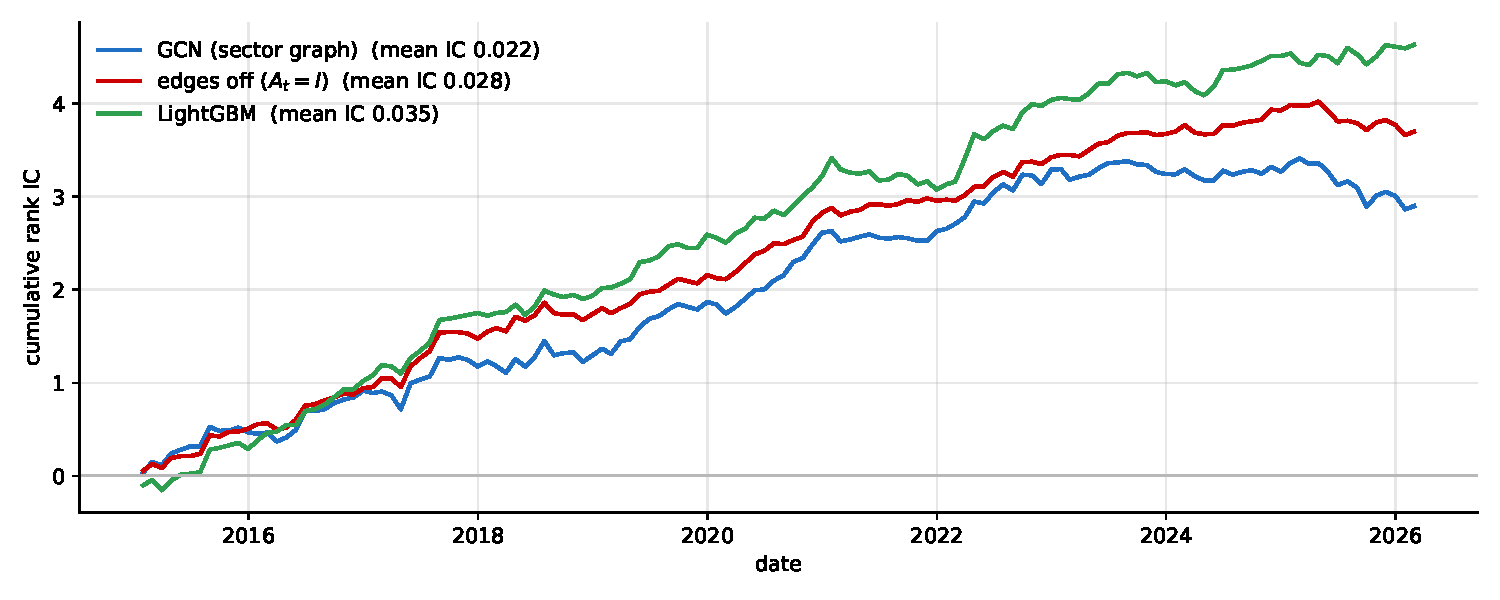
\includegraphics[width=0.7\linewidth]{files/figure_9_2_cumulativ-c0f6718ad81f94f0d78598b5cb722190.pdf}
\caption[]{Cumulative rank information coefficient over the testing period, averaged across five seeds. A rising line indicates a signal that keeps working; the vertical gaps are the cumulative cost of using the graph.}
\label{fig-gnn-cumulative}
\end{figure}

\begin{verbatim}
fig, ax = plt.subplots(figsize=(8, 4))
for i, (name, col) in enumerate([('sector graph', '#1f6fc4'), ('edges off', '#cc0000')]):
    vals = [s.mean() for s in series[name]]
    ax.scatter([i] * len(vals), vals, s=45, color=col, zorder=3)
    ax.hlines(np.mean(vals), i - 0.15, i + 0.15, color='black', lw=2, zorder=4)
ax.axhline(lgb_s.mean(), color='#2e9e4f', ls='--', lw=1.3, label=f'LightGBM ({lgb_s.mean():.4f})')
ax.set_xticks([0, 1]); ax.set_xticklabels(['GCN (sector graph)', 'edges off ($A_t=I$)'])
ax.set_ylabel('average rank IC'); ax.legend(frameon=False)
ax.spines[['top', 'right']].set_visible(False); ax.grid(alpha=.3, axis='y')
plt.tight_layout(); plt.savefig('images/figure_9_3_dispersion.png', dpi=150, bbox_inches='tight')
\end{verbatim}

\begin{figure}[!htbp]
\centering
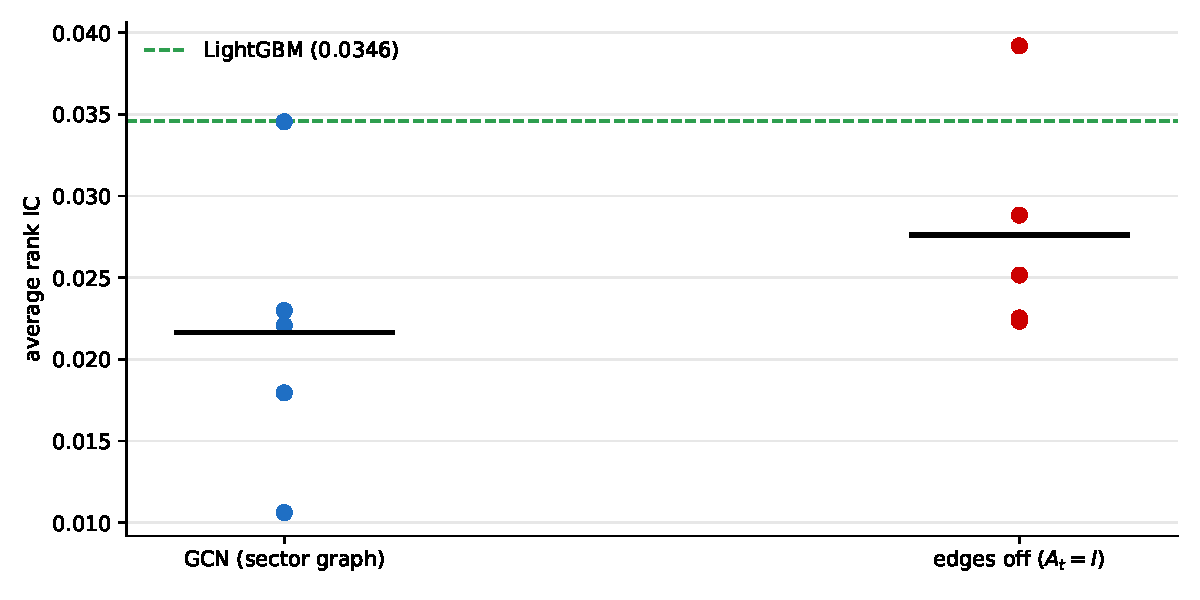
\includegraphics[width=0.7\linewidth]{files/figure_9_3_dispersio-fb54a2eb8780d0ddc05fe33f56526bf6.pdf}
\caption[]{Dispersion of the average rank IC across five random seeds for the sector-graph GCN and its edge-free twin, with the LightGBM benchmark dashed. The seed dispersion is comparable to the gap between the two models.}
\label{fig-gnn-dispersion}
\end{figure}

\paragraph{The ablation, and what survives the noise}\label{sec_gnn_survives}

Because both models are trained under the same five seeds, we difference the graph convolutional network against its own capacity-matched edge-free twin, seed by seed, which cancels the common component of initialisation noise. The twin is the identical class with its neighbourhood aggregation overridden to the identity, so it carries the same architecture and the same 5,025 parameters. Both the paired difference and a time-series test of the monthly gap come straight from the seed-by-seed information coefficients collected above.

\begin{verbatim}
diff = np.array([series['sector graph'][sd].mean() - series['edges off'][sd].mean()
                 for sd in range(5)])                       # paired within each seed
paired_t = diff.mean() / (diff.std(ddof=1) / np.sqrt(len(diff)))
def newey_west_t(x, lags=6):                                # HAC t-statistic for a mean
    x = np.asarray(x, float); n = len(x); e = x - x.mean(); s = e @ e / n
    for l in range(1, lags + 1):
        s += 2 * (1 - l / (lags + 1)) * (e[l:] @ e[:-l]) / n
    return x.mean() / np.sqrt(s / n)
monthly = (mseries['sector graph'] - mseries['edges off']).dropna()   # seed-averaged monthly gap
print(f'GCN minus edge-free twin: mean {diff.mean():+.4f}, '
      f'{int((diff > 0).sum())} of 5 seeds favour the graph, paired t = {paired_t:.2f}')
print(f'same gap over {len(monthly)} months: Newey-West t = {newey_west_t(monthly.values):.2f}')
\end{verbatim}

\begin{verbatim}
GCN minus edge-free twin: mean -0.0060, 0 of 5 seeds favour the graph, paired t = -3.98
same gap over 134 months: Newey-West t = -1.55
\end{verbatim}

TABLE 9.1 records the paired comparison. None of the five seeds favours the graph, and the paired t of -3.98 says the penalty is a stable property of the training procedure, not a lucky draw.

TABLE 9.1: Paired comparison of the graph convolutional network against its capacity-matched edge-free twin. The difference is computed within each seed and then averaged over five seeds. A positive difference would mean the edges add predictive content.

\bigskip\noindent
\begin{tabular}{p{\dimexpr 0.250\linewidth-2\tabcolsep}p{\dimexpr 0.250\linewidth-2\tabcolsep}p{\dimexpr 0.250\linewidth-2\tabcolsep}p{\dimexpr 0.250\linewidth-2\tabcolsep}}
\toprule
Comparison & Mean difference in rank IC & Seeds favouring the graph & Paired t \\
\hline
GCN minus its $\mathbf{A}_t=\mathbf{I}$ twin & -0.0060 & 0 of 5 & -3.98 \\
\bottomrule
\end{tabular}

\bigskip

The result is not special to the graph convolution. Repeating the same ablation for the attention and inductive variants of Section~\ref{sec_gnn_families}, each against its own edge-free twin, returns the same verdict: every architecture loses, with GraphSAGE penalised the least because its separate-then-concatenate design can most easily discount an uninformative neighbourhood, and GATv2 no better off because its attention gate still folds the neighbour average in.

The penalty should not, however, be overstated as a claim about this particular decade. The gap is robust across seeds, with a paired t of -3.98, yet the same monthly differences tested as a 134-month time series with Newey-West standard errors give t = -1.55, within the sampling noise a single backtest carries. Several further checks all point the same way. A range of alternative graphs, from correlation and nearest-neighbour constructions to an external corporate-relations graph, each lose to their own ablation, and the ones whose edges are the purest function of the node features do the most harm. Handing the graph to LightGBM as ordinary features rather than as a structure to propagate over changes nothing, since the 122 characteristics already express the grouping the edges encode. Replacing the averaging with a subtraction, the industry-neutralised peer-relative variant, removes the entire penalty but only recovers the graph-free performance. And net of twenty basis points of costs the graph turns over least yet still nets least. The verdict is therefore narrow and firm: on this panel the sector adjacency carries no incremental information a graph-free model does not already have, and the best a graph does is stop hurting.

\subsubsection{Other families of graph models}\label{sec_gnn_families}

The graph convolution is the simplest aggregator, and the family is larger. We survey the members most relevant to a cross-section of firms, isolating for each the one change it makes to the message-passing rule of equations (9.1) and (9.2), and keeping the treatment brief since none overturns the verdict of Section~\ref{sec_gnn_panel}.

\paragraph{Sampling and attention: GraphSAGE, GAT and GATv2}\label{sec_gnn_sage}

GraphSAGE (\cite{hamilton2017inductive}) departs from the graph convolution in the update step: instead of folding a node and its neighbours into a single weighted average before one linear map, as equation (9.2) does, it keeps the two in separate concatenated slots,

\begin{equation}
\label{eq_gnn_3}
\mathbf{o}_{t,n}^{(l+1)} = f^{(l)}\!\left( \mathbf{W}^{(l)} \left[\, \mathbf{o}_{t,n}^{(l)} \,\Big\|\, \underset{m \in \mathcal{N}(n)}{\mathrm{mean}}\ \mathbf{o}_{t,m}^{(l)} \,\right] \right)
\end{equation}

where $\|$ denotes concatenation and the neighbourhood $\mathcal{N}(n)$ is subsampled to a fixed size, so the cost per node does not grow with degree. Splitting the weight into the block acting on the node and the block acting on its neighbours, $\mathbf{W}^{(l)} = [\,\mathbf{W}^{(l)}_{\mathrm{self}}\ \ \mathbf{W}^{(l)}_{\mathrm{nbr}}\,]$, shows why the design matters here: the network can drive $\mathbf{W}^{(l)}_{\mathrm{nbr}}$ to zero and recover the graph-free map of Section~\ref{sec_gnn_ablation} exactly, discounting an uninformative neighbourhood rather than being forced to average it in. This is the mechanism behind GraphSAGE being the least penalised of the three architectures in Section~\ref{sec_gnn_survives}. Its inductive design, learning a function of a neighbourhood rather than a fixed per-node embedding, is also what lets a model trained on one month's graph apply to the next, whose node set differs.

Graph attention (\cite{velickovic2018graph}) keeps the aggregation of (9.2) but replaces its fixed, degree-based weights with learned, pair-specific ones,

\begin{equation}
\label{eq_gnn_4}
\mathbf{o}_{t,n}^{(l+1)} = f^{(l)}\!\Big( \sum_{m \in \mathcal{N}(n) \cup \{n\}} \alpha_{nm}\, \mathbf{W}^{(l)} \mathbf{o}_{t,m}^{(l)} \Big), \qquad \alpha_{nm} = \mathrm{softmax}_m\big(e_{nm}\big)
\end{equation}

with the score, in the original form, $e_{nm} = \mathrm{LeakyReLU}\big( \mathbf{a}'[\mathbf{W}\mathbf{o}_{t,n} \,\|\, \mathbf{W}\mathbf{o}_{t,m}] \big)$. One line of algebra exposes its flaw. Writing $\mathbf{a} = [\mathbf{a}_1 \,\|\, \mathbf{a}_2]$, the score is $\mathrm{LeakyReLU}\big(\mathbf{a}_1'\mathbf{W}\mathbf{o}_{t,n} + \mathbf{a}_2'\mathbf{W}\mathbf{o}_{t,m}\big)$; for a fixed query node $n$ the first term is constant across the neighbours $m$, and because LeakyReLU is monotone the neighbours are ranked by $\mathbf{a}_2'\mathbf{W}\mathbf{o}_{t,m}$ alone, an ordering that does not depend on $n$. Every node therefore attends to its neighbours in the same order, a static attention that cannot let a bank attend to one set of peers while a miner attends to another. \cite{brody2022attentive} correct this in GATv2 by moving the linear map and the nonlinearity, scoring with $e_{nm} = \mathbf{a}'\,\mathrm{LeakyReLU}\big(\mathbf{W}[\mathbf{o}_{t,n} \,\|\, \mathbf{o}_{t,m}]\big)$, which makes the score a universal approximator of the pair and the attention genuinely dynamic. On our panel GATv2's edges are as costly as the GCN's, and the added expressiveness buys nothing when the graph itself is uninformative.

\paragraph{Sum aggregation and typed edges: GIN and R-GCN}\label{sec_gnn_gin}

The graph isomorphism network of \cite{xu2019powerful} changes the aggregator in (9.1) from a mean to a sum, wrapped in a small multilayer perceptron with a tunable self-weight,

\begin{equation}
\label{eq_gnn_5}
\mathbf{o}_{t,n}^{(l+1)} = \mathrm{MLP}^{(l)}\!\Big( \big(1 + \epsilon^{(l)}\big)\,\mathbf{o}_{t,n}^{(l)} + \sum_{m \in \mathcal{N}(n)} \mathbf{o}_{t,m}^{(l)} \Big).
\end{equation}

The sum is injective on multisets where the mean is not: a neighbourhood $\{\mathbf{a}\}$ and a neighbourhood $\{\mathbf{a}, \mathbf{a}\}$ share a mean but differ in sum, so a mean aggregator cannot tell a node with one such neighbour from a node with two. This is what gives GIN the discriminative power of the Weisfeiler-Lehman graph isomorphism test. The distinction is largely moot here, as the authors themselves note: mean and sum coincide in power once node features are rich and rarely repeat, the situation of a cross-section described by 122 continuous characteristics.

When edges carry types, as in a knowledge graph of supplier, competitor and subsidiary relations, the relational GCN of \cite{schlichtkrull2018modeling} sums a separate transform over each relation,

\begin{equation}
\label{eq_gnn_6}
\mathbf{o}_{t,n}^{(l+1)} = f^{(l)}\!\Big( \mathbf{W}_0^{(l)}\mathbf{o}_{t,n}^{(l)} + \sum_{r \in \mathcal{R}} \sum_{m \in \mathcal{N}_r(n)} \frac{1}{c_{n,r}}\, \mathbf{W}_r^{(l)}\mathbf{o}_{t,m}^{(l)} \Big)
\end{equation}

where $\mathcal{N}_r(n)$ are the neighbours under relation $r$ and $c_{n,r}$ a normaliser; equation (9.2) is the single-relation special case. Because a distinct $\mathbf{W}_r^{(l)}$ per relation is expensive, the relations share a small set of $B$ basis matrices, $\mathbf{W}_r^{(l)} = \sum_{b=1}^{B} a_{rb}^{(l)}\mathbf{V}_b^{(l)}$, which controls the parameter count. It is the natural architecture for external corporate-relation graphs, none of which earned its edges on our data.

\paragraph{Temporal and spatio-temporal graphs}\label{sec_gnn_temporal}

A final family lets the graph, or the model acting on it, evolve, which a monthly panel with a changing node set invites. Where a static GNN applies the same weights at every date, EvolveGCN (\cite{pareja2020evolvegcn}) drives the weight matrix of a graph convolution with a recurrent network,

\begin{equation}
\label{eq_gnn_7}
\mathbf{W}_t^{(l)} = \mathrm{GRU}\big(\mathbf{W}_{t-1}^{(l)},\, \mathbf{H}_t^{(l)}\big)
\end{equation}

so equation (9.2) is applied at each date with weights that carry state across time rather than being refitted independently. The temporal graph attention of \cite{xu2020inductive} instead augments the attention score of (9.4) with a functional encoding of the elapsed time, weighting recent interactions more heavily, and PyTorch Geometric Temporal (\cite{rozemberczki2021pytorch}) makes both accessible. We do not pursue them, for the reason the static results make plain: there is little sense in letting a graph evolve until a static one has been shown to help, and on this panel none has.

\subsubsection{Interpretability}\label{sec_gnn_interp}

If a graph model did produce a useful signal, the natural question is which neighbours and which characteristics produced it. The literature on explaining graph networks, surveyed by \cite{yuan2023explainability}, is organised along three axes worth naming, because each determines what an explanation can and cannot claim. The first is local versus global: a local explanation accounts for a single prediction, one firm on one date, while a global explanation characterises the model's logic across the whole sample, such as the concept a hidden neuron responds to. The second is the instance-level explainer, which for one prediction returns a compact subgraph and a small set of features that suffice to reproduce it. The third, and the most consequential, is intrinsic versus post-hoc: an intrinsically interpretable model builds transparency into its architecture, whereas a post-hoc method probes an already-trained model from outside. A graph convolutional network is not intrinsically interpretable, and attention, the one component that looks as though it might be, is a weak substitute: the debate opened by \cite{jain2019attention} over whether attention weights are explanations is unresolved, and both \cite{ying2019gnnexplainer} and \cite{luo2020parameterized} find an attention baseline the weakest method at recovering structure known to have generated the label.

The standard post-hoc, instance-level tools are therefore the ones to reach for. GNNExplainer (\cite{ying2019gnnexplainer}) learns a soft mask over the edges and node features in a prediction's neighbourhood by maximising the mutual information between the masked input and the model's output. Writing $\mathbf{M}$ for the edge mask, $f$ for the trained network and $\hat{y}$ for its original prediction, this is equivalent to

\begin{equation}
\label{eq_gnn_8}
\min_{\mathbf{M}}\ \ell\big(\hat{y},\, f(\mathcal{G}_{\mathbf{M}})\big) + \lambda \lVert \mathbf{M} \rVert_1, \qquad \mathcal{G}_{\mathbf{M}} = \text{input with edges reweighted by } \sigma(\mathbf{M})
\end{equation}

where the loss $\ell$ keeps the masked prediction close to the original and the $\ell_1$ penalty forces the retained subgraph to be small. Because it re-optimises a mask for every instance, GNNExplainer is purely local and does not transfer. PGExplainer (\cite{luo2020parameterized}) removes that cost by training a single parameterised network that maps edge embeddings to a mask, so one fitted explainer generates explanations for many predictions and, being inductive, extends to nodes it never saw in training, a step from the local toward the global. Feature attributions such as integrated gradients (\cite{sundararajan2017axiomatic}, via the Captum library of \cite{kokhlikyan2020captum}) answer the complementary question of which of the 122 characteristics moved a given forecast. PyTorch Geometric collects these under one interface, the \texttt{torch\_geometric.explain} module of \cite{fey2019fast}, which pairs an explainer algorithm with a common set of evaluation metrics.

Those metrics are what keep the exercise disciplined, and two are standard. Fidelity measures how far the prediction moves when the components an explanation calls important are removed: a faithful explanation should cause a large drop, so high fidelity is the primary evidence that the identified subgraph is the one the model actually used. Sparsity rewards the opposite, an explanation that invokes as few edges and features as possible, on the principle that an account naming half the graph explains nothing. The two are in tension, and a method is judged by the fidelity it retains at a given sparsity. The difficulty is that these benchmarks are themselves fragile: \cite{agarwal2023evaluating} show that on the usual datasets a random explainer can match the published scores, so a good fidelity number is necessary but far from sufficient.

The explainers above act on the edges; the complementary question, which of the 122 characteristics a forecast rests on, has a simple and model-agnostic answer, the permutation importance familiar from the tree ensembles of Chapter 7. We scramble each characteristic across firms within a date, one at a time, and record how far the out-of-sample rank IC falls, so that a large fall marks a characteristic the model relied on. Running this for the sector-graph GCN and its edge-free twin, on the fixed pre-2015 training split of Figure~\ref{fig-gnn-depth}, asks not merely what the model uses but whether the graph changes it.

\begin{verbatim}
set_seed(SEED)
m_graph = fit_gnn(lambda: DeepGCN(K, 32, 2), tr_fix)         # trained sector-graph GCN
m_free  = fit_gnn(lambda: DeepGCN_NoGraph(K, 32, 2), tr_fix) # its edge-free twin

def perm_importance(model, snaps):                          # drop in rank IC when a characteristic is scrambled
    rng = np.random.default_rng(SEED)
    base = np.nanmean([spearmanr(model(X, sec).detach().numpy(), raw).statistic for _, X, _, sec, raw in snaps])
    imp = np.zeros(K)
    for k in range(K):
        ics = []
        for _, X, _, sec, raw in snaps:
            Xp = X.clone(); Xp[:, k] = X[torch.tensor(rng.permutation(X.size(0))), k]   # shuffle within the date
            ics.append(spearmanr(model(Xp, sec).detach().numpy(), raw).statistic)
        imp[k] = base - np.nanmean(ics)
    return imp

imp_g, imp_f = perm_importance(m_graph, te_fix), perm_importance(m_free, te_fix)
rho = spearmanr(imp_g, imp_f).statistic
top = np.argsort(-imp_g)[:15]                               # the fifteen the graph model leans on most
print(f'importance rank correlation, graph vs edges off: {rho:.2f}')
for k in top:
    print(f'{features[k]:<24}graph {imp_g[k]:+.4f}   edges off {imp_f[k]:+.4f}')
\end{verbatim}

\begin{verbatim}
importance rank correlation, graph vs edges off: 0.57
Book_Value_PS           graph +0.0036   edges off +0.0029
REV_Quarterly_Surprise  graph +0.0024   edges off +0.0023
rsi_14                  graph +0.0022   edges off +0.0014
mom_252                 graph +0.0021   edges off +0.0021
rel_str_252d            graph +0.0017   edges off +0.0027
vol_22                  graph +0.0016   edges off +0.0028
Mom_Sharp_11M           graph +0.0016   edges off +0.0036
Asset_Turn              graph +0.0014   edges off +0.0005
EPS_FY1_Rev30d          graph +0.0013   edges off +0.0020
Dividend_Payout_Ratio   graph +0.0011   edges off +0.0000
OCF_to_NOA              graph +0.0010   edges off +0.0010
size_log                graph +0.0010   edges off +0.0007
vol_66                  graph +0.0009   edges off +0.0022
EV_Sales                graph +0.0009   edges off -0.0008
dd                      graph +0.0008   edges off +0.0023
\end{verbatim}

\begin{verbatim}
top15 = np.argsort(imp_g)[-15:]                            # ascending, bottom-to-top in the bar chart
fig, ax = plt.subplots(1, 2, figsize=(12, 5), gridspec_kw={'width_ratios': [1.5, 1]})
y = np.arange(len(top15))
ax[0].barh(y + 0.2, imp_g[top15], height=0.4, color='#1f6fc4', label='sector graph')
ax[0].barh(y - 0.2, imp_f[top15], height=0.4, color='#cc0000', label='edges off ($A_t=I$)')
ax[0].set_yticks(y); ax[0].set_yticklabels(np.array(features)[top15], fontsize=8)
ax[0].axvline(0, color='#b8b8b8', lw=.8); ax[0].set_xlabel('drop in rank IC when scrambled')
ax[0].legend(frameon=False, loc='lower right'); ax[0].spines[['top', 'right']].set_visible(False)
lo, hi = min(imp_g.min(), imp_f.min()), max(imp_g.max(), imp_f.max())
ax[1].plot([lo, hi], [lo, hi], color='#b8b8b8', lw=1)
ax[1].scatter(imp_f, imp_g, s=20, color='#6a3d9a', alpha=.75, edgecolor='none')
ax[1].set_xlabel('importance, edges off'); ax[1].set_ylabel('importance, sector graph')
ax[1].set_title(f'all 122 characteristics  ($\\rho$ = {rho:.2f})', fontsize=10)
ax[1].spines[['top', 'right']].set_visible(False)
plt.tight_layout(); plt.savefig('images/figure_9_4_importance.png', dpi=150, bbox_inches='tight')
\end{verbatim}

\begin{figure}[!htbp]
\centering
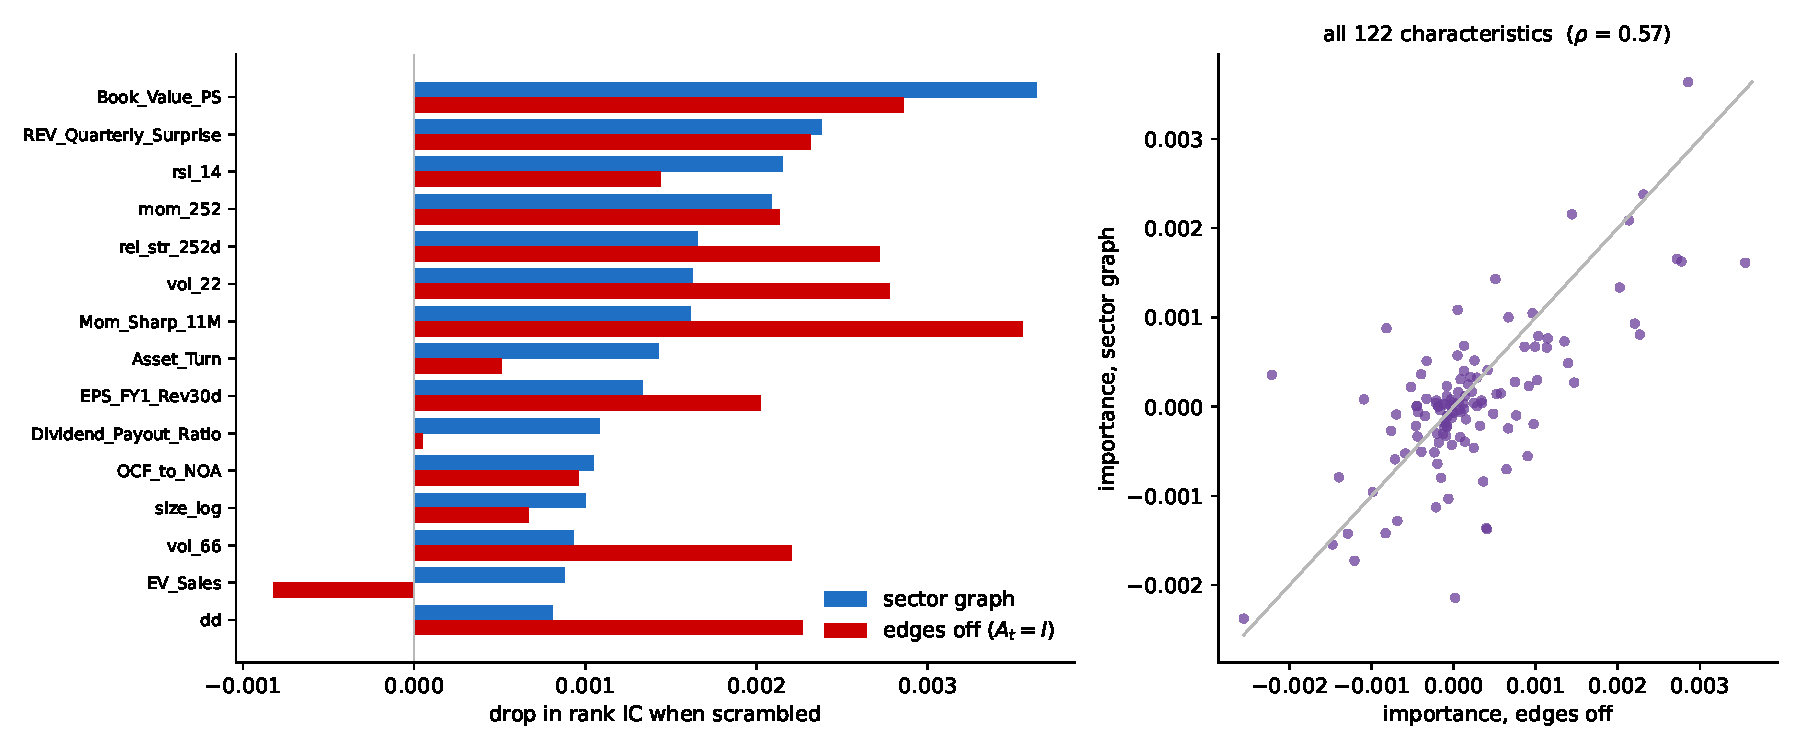
\includegraphics[width=0.7\linewidth]{files/figure_9_4_importanc-91b9b860bde5bf329c185f81ae3e8389.pdf}
\caption[]{Permutation importance of the 122 characteristics for the sector-graph GCN and its edge-free twin, on the fixed 2015 split. Left: the fifteen characteristics the graph model relies on most, measured by the drop in out-of-sample rank IC when each is scrambled within its date. Right: the importance of every characteristic under the graph against its importance without it, with Spearman correlation $\rho$.}
\label{fig-gnn-importance}
\end{figure}

\subsubsection{Coding exercises}\label{sec_gnn_exercises}

\begin{enumerate}
\item Compute the edge homophily ratio for a graph built from the finer NAICS subsector code rather than the sector code, and compare it with the sector value of 0.607. Does a narrower industry definition raise homophily, and does a GCN trained on it do any better against its edge-free twin?
\item Replace the sector graph by a correlation graph, connecting each firm to the ten others whose returns were most correlated over the preceding twelve months. Verify that the construction uses no information posterior to the formation date, and comment on the month-to-month turnover of the edge set.
\end{enumerate}

\subsubsection{References}